% Options for packages loaded elsewhere
\PassOptionsToPackage{unicode}{hyperref}
\PassOptionsToPackage{hyphens}{url}
%
\documentclass[
]{article}
\usepackage{lmodern}
\usepackage{amssymb,amsmath}
\usepackage{ifxetex,ifluatex}
\ifnum 0\ifxetex 1\fi\ifluatex 1\fi=0 % if pdftex
  \usepackage[T1]{fontenc}
  \usepackage[utf8]{inputenc}
  \usepackage{textcomp} % provide euro and other symbols
\else % if luatex or xetex
  \usepackage{unicode-math}
  \defaultfontfeatures{Scale=MatchLowercase}
  \defaultfontfeatures[\rmfamily]{Ligatures=TeX,Scale=1}
\fi
% Use upquote if available, for straight quotes in verbatim environments
\IfFileExists{upquote.sty}{\usepackage{upquote}}{}
\IfFileExists{microtype.sty}{% use microtype if available
  \usepackage[]{microtype}
  \UseMicrotypeSet[protrusion]{basicmath} % disable protrusion for tt fonts
}{}
\makeatletter
\@ifundefined{KOMAClassName}{% if non-KOMA class
  \IfFileExists{parskip.sty}{%
    \usepackage{parskip}
  }{% else
    \setlength{\parindent}{0pt}
    \setlength{\parskip}{6pt plus 2pt minus 1pt}}
}{% if KOMA class
  \KOMAoptions{parskip=half}}
\makeatother
\usepackage{xcolor}
\IfFileExists{xurl.sty}{\usepackage{xurl}}{} % add URL line breaks if available
\IfFileExists{bookmark.sty}{\usepackage{bookmark}}{\usepackage{hyperref}}
\hypersetup{
  pdftitle={Discrete Choice Modeling},
  hidelinks,
  pdfcreator={LaTeX via pandoc}}
\urlstyle{same} % disable monospaced font for URLs
\usepackage[margin=1in]{geometry}
\usepackage{longtable,booktabs}
% Correct order of tables after \paragraph or \subparagraph
\usepackage{etoolbox}
\makeatletter
\patchcmd\longtable{\par}{\if@noskipsec\mbox{}\fi\par}{}{}
\makeatother
% Allow footnotes in longtable head/foot
\IfFileExists{footnotehyper.sty}{\usepackage{footnotehyper}}{\usepackage{footnote}}
\makesavenoteenv{longtable}
\usepackage{graphicx,grffile}
\makeatletter
\def\maxwidth{\ifdim\Gin@nat@width>\linewidth\linewidth\else\Gin@nat@width\fi}
\def\maxheight{\ifdim\Gin@nat@height>\textheight\textheight\else\Gin@nat@height\fi}
\makeatother
% Scale images if necessary, so that they will not overflow the page
% margins by default, and it is still possible to overwrite the defaults
% using explicit options in \includegraphics[width, height, ...]{}
\setkeys{Gin}{width=\maxwidth,height=\maxheight,keepaspectratio}
% Set default figure placement to htbp
\makeatletter
\def\fps@figure{htbp}
\makeatother
\setlength{\emergencystretch}{3em} % prevent overfull lines
\providecommand{\tightlist}{%
  \setlength{\itemsep}{0pt}\setlength{\parskip}{0pt}}
\setcounter{secnumdepth}{-\maxdimen} % remove section numbering

\title{Discrete Choice Modeling}
\usepackage{etoolbox}
\makeatletter
\providecommand{\subtitle}[1]{% add subtitle to \maketitle
  \apptocmd{\@title}{\par {\large #1 \par}}{}{}
}
\makeatother
\subtitle{USP 657}
\author{}
\date{\vspace{-2.5em}21 June, 2020}

\begin{document}
\maketitle

\hypertarget{section}{%
\section{}\label{section}}

\hypertarget{sic}{%
\subsection{SIC}\label{sic}}

\texttt{A\ Self\ Instructing\ Course\ in\ Mode\ Choice\ Modeling:\ Multinomial\ and\ Nested\ Logit\ Models}

\hypertarget{introduction}{%
\subsubsection{1 Introduction}\label{introduction}}

\hypertarget{elements-of-the-choice-decision-process}{%
\subsubsection{2 Elements of the choice decision
process}\label{elements-of-the-choice-decision-process}}

\hypertarget{utility-based-choice-theory}{%
\subsubsection{3 Utility-based choice
theory}\label{utility-based-choice-theory}}

\hypertarget{the-multinomial-logit-model}{%
\subsubsection{4 The Multinomial Logit
Model}\label{the-multinomial-logit-model}}

\hypertarget{extreme-value-type-i-distribution}{%
\paragraph{Extreme Value Type I
Distribution}\label{extreme-value-type-i-distribution}}

The extreme value type I distribution has two forms. One is based on the
smallest extreme and the other is based on the largest extreme. We call
these the minimum and maximum cases, respectively. Formulas and plots
for both cases are given. The extreme value type I distribution is also
referred to as the
\href{https://www.itl.nist.gov/div898/handbook/eda/section3/eda366g.htm}{Gumbel
distribution}.

\begin{longtable}[]{@{}lllll@{}}
\toprule
\begin{minipage}[b]{0.07\columnwidth}\raggedright
\strut
\end{minipage} & \begin{minipage}[b]{0.20\columnwidth}\raggedright
general (minimum)\strut
\end{minipage} & \begin{minipage}[b]{0.20\columnwidth}\raggedright
standard(minimum)\strut
\end{minipage} & \begin{minipage}[b]{0.20\columnwidth}\raggedright
general (maximum)\strut
\end{minipage} & \begin{minipage}[b]{0.20\columnwidth}\raggedright
standard(maximum)\strut
\end{minipage}\tabularnewline
\midrule
\endhead
\begin{minipage}[t]{0.07\columnwidth}\raggedright
\(f(x)\)\strut
\end{minipage} & \begin{minipage}[t]{0.20\columnwidth}\raggedright
\(\frac{1} {\beta} e^{\frac{x-\mu}{\beta}}e^{-e^{\frac{x-\mu}{\beta}}}\)\strut
\end{minipage} & \begin{minipage}[t]{0.20\columnwidth}\raggedright
\(e^{x}e^{-e^{x}}\)\strut
\end{minipage} & \begin{minipage}[t]{0.20\columnwidth}\raggedright
\(\frac{1}{\beta} e^{-\frac{x-\mu}{\beta}}e^{-e^{-\frac{x-\mu}{\beta}}}\)\strut
\end{minipage} & \begin{minipage}[t]{0.20\columnwidth}\raggedright
\(e^{-x}e^{-e^{-x}}\)\strut
\end{minipage}\tabularnewline
\begin{minipage}[t]{0.07\columnwidth}\raggedright
\(F(x)\)\strut
\end{minipage} & \begin{minipage}[t]{0.20\columnwidth}\raggedright
\strut
\end{minipage} & \begin{minipage}[t]{0.20\columnwidth}\raggedright
\(1 - e^{-e^{x}}\)\strut
\end{minipage} & \begin{minipage}[t]{0.20\columnwidth}\raggedright
\strut
\end{minipage} & \begin{minipage}[t]{0.20\columnwidth}\raggedright
\(e^{-e^{-x}}\)\strut
\end{minipage}\tabularnewline
\bottomrule
\end{longtable}

where \(\mu\) is the location parameter and \(\beta\) is the scale
parameter.

Mean \(\mu + 0.5772\beta\) (Euler's number)

Median \(\mu - \beta\ln(\ln(2))\)

Mode \(\mu\)

Range \(-\infty \mbox{ to } \infty\)

Standard Deviation \(\frac{\beta\pi} {\sqrt{6}}\)

Skewness 1.13955

Kurtosis 5.4

Coefficient of Variation
\(\frac {\beta\pi} {\sqrt{6}(\mu + 0.5772\beta)}\)

\begin{longtable}[]{@{}ll@{}}
\toprule
Gumbel\_pmf & Gumbel\_cdf\tabularnewline
\midrule
\endhead
\includegraphics{https://upload.wikimedia.org/wikipedia/commons/thumb/3/32/Gumbel-Density.svg/600px-Gumbel-Density.svg.png}
&
\includegraphics{https://upload.wikimedia.org/wikipedia/commons/thumb/7/7d/Gumbel-Cumulative.svg/600px-Gumbel-Cumulative.svg.png}\tabularnewline
\bottomrule
\end{longtable}

\hypertarget{data-assembly-and-estimation-of-sample-multinomial-logit-model}{%
\subsubsection{5 : Data Assembly and Estimation of sample Multinomial
Logit
Model}\label{data-assembly-and-estimation-of-sample-multinomial-logit-model}}

\hypertarget{data-requirements-overview}{%
\paragraph{5.2 Data requirements
Overview}\label{data-requirements-overview}}

Dependent, endogenous variable: mode choice

Independent, exogenous variables:(automobile ownership, time of day of
travel, origin and destination of trip, and travel party size)

\begin{itemize}
\tightlist
\item
  Traveler related variables
\end{itemize}

Income, Number of automobiles in traveler's household, Number of workers
in traveler's household, Sex, Age, Functions of these variables such as
number of autos divided by number of workers

\begin{itemize}
\tightlist
\item
  Trip context variables
\end{itemize}

Trip purpose, Employment density at the traveler's workplace, Population
density at the home location, and Dummy variable indicating whether the
traveler;s workplace is the Central Business District (CBD)

\begin{itemize}
\tightlist
\item
  Mode (alternative) related variables:
\end{itemize}

Total travel time, IN-vehicle travel time, Out-of-vehicle travel time,
Walk time, Wait time, Number of transfers, Transit headway(service
frequency for carrier modes), and travel cost.

\begin{itemize}
\tightlist
\item
  Interaction of Mode and Traveler or Trip Related Variables
\end{itemize}

Travel cost divided by household income, Travel time or cost interacted
with sex or age group for traveler, and Out-of-Vehicle time divided by
total trip distance.

\hypertarget{sources-and-methods-for-traveler-and-trip-related-data-collection}{%
\paragraph{5.3 Sources and Methods for Traveler and Trip Related Data
Collection}\label{sources-and-methods-for-traveler-and-trip-related-data-collection}}

\begin{itemize}
\tightlist
\item
  Travel Survey Types
\end{itemize}

Household Travel Surveys, Workplace Surveys, Destination Surveys,
Intercept Surveys,

\begin{itemize}
\tightlist
\item
  Sampling Design Considerations
\end{itemize}

Population of interest; Sampling units; The probability sampling;
stratified random sampling; Sample size.

\hypertarget{methods-for-collecting-mode-related-data}{%
\paragraph{5.4 Methods for collecting mode related
data}\label{methods-for-collecting-mode-related-data}}

Network analysis

\hypertarget{data-structure-for-estimation}{%
\paragraph{5.5 Data structure for
estimation}\label{data-structure-for-estimation}}

The trip format: IDCase, each record contains all the information for
mode choice over laternatives for a signle trip.

The trip-alternative format: IDCase-IDAlt, each record contains all the
information for a single mode available to each trip maker so there is
one record for each mode for each trip.

\hypertarget{application-data-for-work-mode-choice-in-the-san-francisco-bay-area}{%
\paragraph{5.6 Application data for work mode choice in the San
Francisco Bay
Area}\label{application-data-for-work-mode-choice-in-the-san-francisco-bay-area}}

\hypertarget{estimation-of-mnl-model-with-basic-specification}{%
\paragraph{5.7 Estimation of MNL Model with Basic
Specification}\label{estimation-of-mnl-model-with-basic-specification}}

\(\begin{aligned} V_{DA}=& &\beta_1TT_{DA}+\beta_2TC_{DA}&\\ V_{SR2}=&\beta_{SR2}+&\beta_1TT_{SR2}+\beta_2TC_{SR2}&+\gamma_{SR2}Inc\\ V_{SR3+}=&\beta_{SR3+}+&\beta_1TT_{SR3+}+\beta_2TC_{SR3+}&+\gamma_{SR3+}Inc\\ V_{TR}=&\beta_{TR}+&\beta_1TT_{TR}+\beta_2TC_{TR}&+\gamma_{TR}Inc\\ V_{BK}=&\beta_{BK}+&\beta_1TT_{BK}+\beta_2TC_{BK}&+\gamma_{BK}Inc\\ V_{WK}=&\beta_{WK}+&\beta_1TT_{WK}+\beta_2TC_{WK}&+\gamma_{WK}Inc \end{aligned}\)

\begin{itemize}
\tightlist
\item
  Informal Tests
\end{itemize}

The sign of parameters (do the associated variables have a positive or
negative effect on the alternatives with which they are associated?),

The difference (positive or negative) within sets of alternative
specific variables (does the inclusion of this variable have a more or
less positive effect on one alternative relative to another?) and

The ratio of pairs of parameters (is the ratio between the parameters of
the correct sign and in a reasonable range?).

\begin{itemize}
\tightlist
\item
  Overall Goodness-of-Fit Measures
\end{itemize}

\(\rho_0^2=1-\frac{LL(\hat\beta)}{LL(0)};\quad\bar\rho_0^2=1-\frac{LL(\hat\beta)-K}{LL(0)}\)

\(\rho_c^2=1-\frac{LL(\hat\beta)}{LL(c)};\quad\bar\rho_c^2=1-\frac{LL(\hat\beta)-K}{LL(c)-K_{MS}}\)

\begin{itemize}
\tightlist
\item
  t test:
\end{itemize}

\texttt{Table\ 5-4\ p.86}

Test of Individual Parameters \(\frac{\hat\beta_k-\beta^*_k}{S_k}\)

Test of Linear Relationship between Parameters \(H_0:\beta_k=\beta_l\),
\(\frac{\hat\beta_k-\hat\beta_l}{\sqrt{S_k^2+S_l^2-2S_{k,l}}}\)

\(H_0:\beta_{cost}=(VOT)\beta_{time}\),
\(\frac{\hat\beta_{cost}-(VOT)\hat\beta_{time}}{\sqrt{S_{cost}^2+(VOT)^2S^2_{time}-2S_{time,cost}}}\)

Tests of Entire Models: LRT \(-2[LL_{R}-LL_U]\)

\texttt{5.7.3.4} The non-nested hypothesis test uses the adjusted
likelihood ratio index \(\bar\rho^2\) to test the hypothesis that the
model with the lower \(\bar\rho^2\) value is the true model

\(\alpha=\Phi[-(-2(\bar\rho^2_H-\bar\rho^2_L)LL(0)+(K_H-K_l))^{\frac12}]\)

\hypertarget{value-of-time}{%
\paragraph{5.8 Value of Time}\label{value-of-time}}

\begin{itemize}
\tightlist
\item
  Value of Time for linear Utility Function
\end{itemize}

\(V_i=...+\beta_{TVT}TVT_i+\beta_{cost}Cost_i+...=...+\beta_{TVT}TVT_{it}+\beta_{costInc}\frac{Cost_{it}}{Income_t}+...\)

\(VofT=\beta_{TVT}/\beta_{cost}=\frac{\partial V_i/\partial Time_i}{\partial V_i/\partial Cost_i}=\frac{\beta_{TVT}}{\beta_{CostInc}/Income_t}\)

\(VofT=\frac{0.6\frac{\beta_{TVT}}{\beta_{Cost}}}{\ln[Income(\frac{\$1000}{year})]}\$/hour\)

\(VofT=\frac{\beta_{TVT}}{\beta_{CostInc}}Units_{VofT}=\frac{\beta_{TVT}}{\beta_{CostInc}}\frac{\frac{cents}{minute}}{\frac{\$1000}{year}}=\frac{\beta_{TVT}}{\beta_{CostInc}}1.2\)

\begin{itemize}
\tightlist
\item
  Value of Time for Time or Cost Transformation
\end{itemize}

\(V_{it}=...+\beta_{\ln(TVT)}\ln(TVT_{it})+\beta_{cost}Cost_{it}+...\)

\(VofT=\frac{\beta_{\ln(TVT)}}{\beta_{Cost}}\frac1{TVT_{it}}=\frac{\beta_{TVT}}{\beta_{\ln(Cost)}}Cost_{it}\)

\hypertarget{section-1}{%
\subsubsection{6}\label{section-1}}

extends this example to the estimation of more sophisticated models.

\hypertarget{section-2}{%
\subsubsection{7}\label{section-2}}

develops a parallel example for shop/other mode choice in the San
Francisco Bay Region.

\hypertarget{nested-logit-model}{%
\subsubsection{8 Nested Logit Model}\label{nested-logit-model}}

\(\begin{align*} U_{DA}=&V_{DA} &&&+&\varepsilon_{DA}\\ U_{SR}=&V_{GRP}+V_{SR} &+\varepsilon_{GRP}&&+&\varepsilon_{SR}\\ U_{Bus}=&V_{GRP}+V_{PT}+V_{Bus}&+\varepsilon_{GRP}&+\varepsilon_{PT}&+&\varepsilon_{Bus}\\ U_{LTR}=&V_{GRP}+V_{PT}+V_{LTR}&+\varepsilon_{GRP}&+\varepsilon_{PT}&+&\varepsilon_{LTR} \end{align*}\)

\(Pr(Bus|PT)=\frac{\exp{(\frac{V_{Bus}}{\theta_{PT}})}}{\exp{(\frac{V_{Bus}}{\theta_{PT}})}+\exp{(\frac{V_{LTR}}{\theta_{PT}})}}\),\(Pr(LTR|PT)=\frac{\exp{(\frac{V_{LTR}}{\theta_{PT}})}}{\exp{(\frac{V_{Bus}}{\theta_{PT}})}+\exp{(\frac{V_{LTR}}{\theta_{PT}})}}\)

\(Pr(SR|GRP)=\frac{\exp{(\frac{V_{SR}}{\theta_{GRP}})}}{\exp{(\frac{V_{SR}}{\theta_{GRP}})}+\exp{(\frac{V_{PT}+\theta_{PT}\Gamma_{PT}}{\theta_{GRP}})}}\),
\(Pr(PT|GRP)=\frac{\exp{(\frac{V_{PT}+\theta_{PT}\Gamma_{PT}}{\theta_{GRP}})}}{\exp{(\frac{V_{SR}}{\theta_{GRP}})}+\exp{(\frac{V_{PT}+\theta_{PT}\Gamma_{PT}}{\theta_{GRP}})}}\),
\(\Gamma_{PT}=\log[\exp{(\frac{V_{Bus}}{\theta_{PT}})}+\exp{(\frac{V_{LTR}}{\theta_{PT}})}]\)

\(Pr(DA)=\frac{\exp{(V_{DA})}}{\exp{(V_{DA})}+\exp{(V_{GRP}+\theta_{GRPT}\Gamma_{GRP})}}\),
\(Pr(GRP)=\frac{\exp{(V_{GRP}+\theta_{GRPT}\Gamma_{GRP})}}{\exp{(V_{DA})}+\exp{(V_{GRP}+\theta_{GRPT}\Gamma_{GRP})}}\),
\(\Gamma_{GRP}=\log[\exp{(\frac{V_{SR}}{\theta_{GRP}})}+\exp{(\frac{V_{PT}+\theta_{PT}\Gamma_{PT}}{\theta_{GRP}})}]\)

\(Pr(SR)=Pr(SR|GRP)Pr(GRP)\)

\(Pr(Bus)=Pr(Bus|PT)Pr(PT|GRP)Pr(GRP)\)

\(Pr(LTR)=Pr(LTR|PT)Pr(PT|GRP)Pr(GRP)\)

\(Var(\varepsilon_{DA})=Var(\varepsilon_{SR})+Var(\varepsilon_{GRP})=Var(\varepsilon_{GRP})+Var(\varepsilon_{PT})+Var(\varepsilon_{Bus})=Var(\varepsilon_{GRP})+Var(\varepsilon_{PT})+Var(\varepsilon_{LTR})=\frac{\pi^2}{6}\),

\(Var(\varepsilon_{Bus})=Var(\varepsilon_{LTR})=\frac{\pi^2}{6\mu_{PT}^2}=\frac{\pi^2\theta^2_{PT}}{6}\),

\(Var(\varepsilon_{GRP})=\frac{\pi^2\theta^2_{Grp}}{6}\),\(Var(\varepsilon_{PT})=\frac{\pi^2\theta^2_{PT}}{6}\),
\(Var(\varepsilon_{Total}-\varepsilon_{GRP})=\frac{\pi^2}{6}(1-\theta^2_{Grp})\),\(Var(\varepsilon_{Grp}-\varepsilon_{PT})=\frac{\pi^2}{6}(\theta^2_{Grp}-\theta^2_{PT})\)

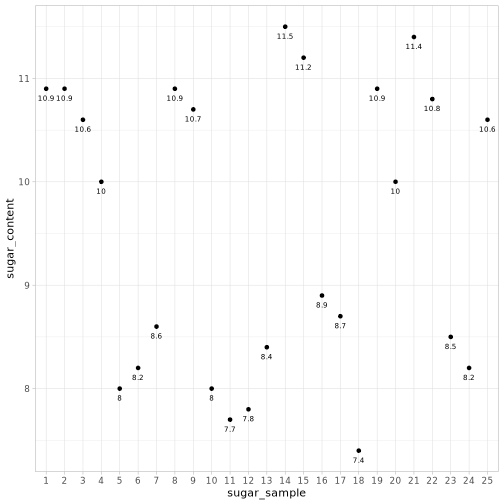
\includegraphics[width=0.5\linewidth]{note_usp657_files/figure-latex/unnamed-chunk-1-1}

Adopting a nested logit model implies rejection of the MNL

\(Var(\varepsilon_{LTR}^*)=Var(\varepsilon_{GRP})+Var(\varepsilon_{PT})+Var(\varepsilon_{LTR})=\frac{\pi^2}{6}\),

\hypertarget{selecting-a-preferred-nesting-structure}{%
\subsubsection{9 Selecting a Preferred Nesting
Structure}\label{selecting-a-preferred-nesting-structure}}

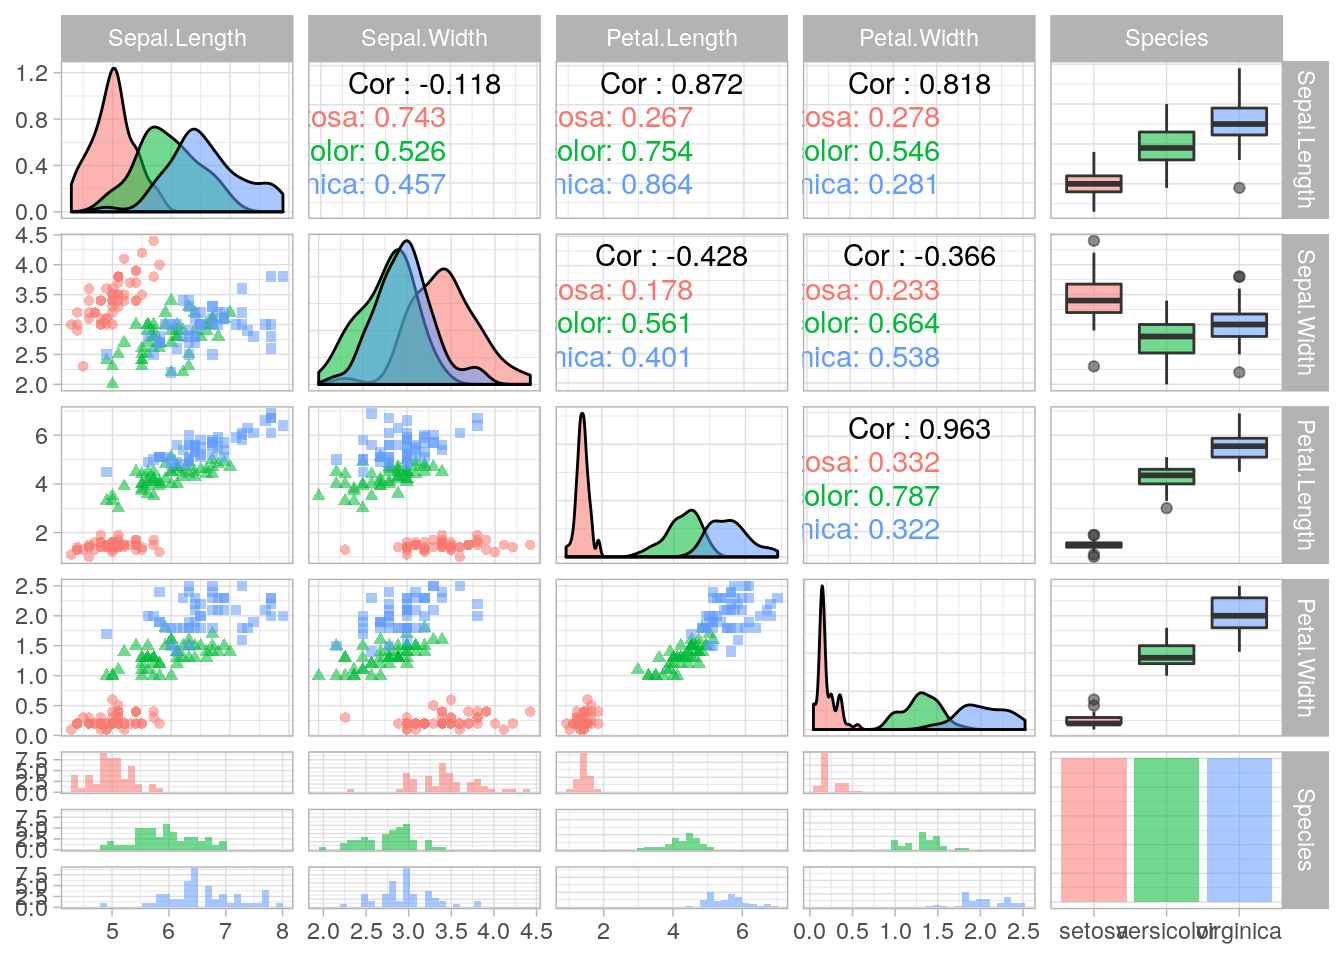
\includegraphics[width=0.5\linewidth]{note_usp657_files/figure-latex/unnamed-chunk-2-1}

\hypertarget{multiple-maxima-in-the-estimation-of-nested-logit-models}{%
\subsubsection{10 Multiple Maxima in the Estimation of Nested Logit
Models}\label{multiple-maxima-in-the-estimation-of-nested-logit-models}}

\hypertarget{aggregate-forecasting-assessment-and-application}{%
\subsubsection{11 Aggregate Forecasting, Assessment, and
Application}\label{aggregate-forecasting-assessment-and-application}}

\hypertarget{aggregate-forecasting}{%
\paragraph{11.2 Aggregate Forecasting}\label{aggregate-forecasting}}

\(\hat N_i=\sum_{n=1}^NP_i(x_{ni},\hat\theta)=\sum_{n=1}^N\hat P_{ni}\)

Where \(\theta\) is the expected value of the vector of parameters
obtained in the estimation phase and \(\hat P_{ni}\) is the estimated
probability of choosing mode \(i\) for individual \(n\).

\(\hat S_i=\frac1N\sum_{n=1}^NP_i(x_{ni},\hat\theta)=\frac1N\sum_{n=1}^N\hat P_{ni}\)

Two sources of variation:

the probabilistic form of the discrete choice model at the individual
level. This sampling variance declines with the size \(N\) of the
population for which an aggregate prediction is desired. \(N\) is likely
to be large enough so that the sampling variance can be ignored.

An estimate vector \(\hat\theta\) of the true value. An estimate of the
asymptotic variance of the aggregate share prediction due to this
estimation variance:

\(Var(\hat S_i)=d_i'Var(\hat\theta)d_i\), where
\(d_i=\frac1N\sum_{n=1}^N[\hat P_{ni}(x_{ni}-\sum_j\hat P_{nj}x_{nj})]\)

\(Var(\hat\theta)\) is the asymptotic variance-covariance matrix of the
parameters obtained in estimation and \(d_i'\) is the transpose matrix
of \(d_i\). If the dimension of the vector \(x_{ni}\) is \(K\times1\),
then the dimension of \(d_i\) is also \(K\times1\) and the dimension of
\(Var(\hat\theta)\) is \(K\times K\).

sample enumeration: uses a random sample of the population of interest
and then applies equation to the sample.

synthetic population:construct a synthetic prediction sample for the
entire population through micro-simulation.

\(\tilde S_i=\frac1M\sum_{n=1}^MP_i(x_{ni},\hat\theta)=\frac1M\sum_{n=1}^M\hat P_{ni}\)

A two-step iterative proportional fitting (IPF) procedure is used to
estimate simultaneously the multi-way distribution for each census tract
within a PUMA (Miller, 1996), in such a way as to match the marginal
distribution of each census tract and the multi-way correlation of the
PUMA(Public Use Microdata Area) in the Public Use Microdata Sample
(PUMS).

\hypertarget{aggregate-assessment-of-travel-mode-choice-models}{%
\paragraph{11.3 Aggregate Assessment of Travel Mode Choice
Models}\label{aggregate-assessment-of-travel-mode-choice-models}}

The testing of alternative model structures and specifications should be
conducted at the disaggregate level to select a preferred model
structure/specification. This testing and selection process should not
be pursued at the aggregate level.

\begin{enumerate}
\def\labelenumi{\arabic{enumi}.}
\item
  In some model structures such as the multinomial logit, the predicted
  aggregate share of each modal alternative in the estimation sample
  will be the same regardless of the model specification as long as a
  full set of alternative specific constants are included. Thus,
  aggregate testing of alternative models using the estimation sample is
  futile.
\item
  A model that performs poorly at the disaggregate level may perform as
  well or even better than a model that performs well at the
  disaggregate level when both models are applied to a hold-out sample
  to obtain aggregate predictions.
\item
  errors in individual-level predictions tend to average out in the
  aggregate, and so aggregate-level testing does not discriminate much
  among alternative models.
\item
  the same problems mentioned earlier are applicable (though to a lesser
  extent) even for semi-aggregate comparisons among alternative models.
\end{enumerate}

Once a model has been selected, it becomes necessary to validate the
models at the aggregate level. This validation is used to ensure that
the prediction of aggregate behavior, which drives the modeling process,
is consistent with the historically observed aggregate data and by
extension future aggregate behavior. Effective validation requires
matching prediction to observations at easily observable and measurable
locations.

The predicted shares can be compared to the actual shares and summary
measures such as the root mean square error or average absolute error
percentage may be computed to assess the degree to which the predictions
correspond to the aggregate observed data.

\hypertarget{recent-advances-in-discrete-choice-modeling}{%
\subsubsection{12 Recent Advances in Discrete Choice
Modeling}\label{recent-advances-in-discrete-choice-modeling}}

(Bhat, 2005) The first assumption in the MNL model is that the random
components of the utilities of the different alternatives are
independent and identically distributed (IID).

The assumption of \emph{independence} implies that there are no common
unobserved factors affecting the utilities of the various alternatives.
The same underlying unobserved factor (opportunity to socialize or lack
of privacy) impacts the utilities of multiple modes. The presence of
such common underlying factors across modal utilities has implications
for competitive structure.

The assumption of \emph{identically} distributed (across alternatives)
random utility terms implies that the variation in unobserved factors
affecting modal utility is the same across all modes. If comfort is an
unobserved variable whose values vary considerably for the train mode
but little for the automobile mode, then the random components for the
automobile and train modes will have different variances. Unequal error
variances have significant implications for competitive structure, as
discussed in detail by Bhat (1995).

A second assumption of the MNL model is that it maintains
\emph{homogeneity} in responsiveness to attributes of alternatives
across individuals

The MNL model does not allow sensitivity variations to an attribute (for
example, travel cost or travel time in a mode choice model) due to
unobserved individual characteristics. However, unobserved individual
characteristics can and generally will affect responsiveness. Ignoring
the effect of unobserved individual attributes can lead to biased and
inconsistent parameter and choice probability estimates (see
Chamberlain, 1980).

\hypertarget{the-gev-class-of-models}{%
\paragraph{12.2 The GEV Class of Models}\label{the-gev-class-of-models}}

The GEV-class of models relaxes the independence from irrelevant
alternatives (IIA) property of the multinomial logit model by relaxing
the independence assumption between the error terms of alternatives. In
other words, a generalized extreme value error structure is used to
characterize the unobserved components of utility as opposed to the
univariate and independent extreme value error structure used in the
multinomial logit model.

three important characteristics of all GEV models:

\begin{enumerate}
\def\labelenumi{(\arabic{enumi})}
\item
  the overall variances of the alternatives (i.e., the scale of the
  utilities of alternatives) are assumed to be identical across
  alternatives,
\item
  the choice probability structure takes a closed-form expression, and
\item
  all GEV models collapse to the MNL model when the parameters
  generating correlation take values that reduce the correlations
  between each pair of alternatives to zero.
\end{enumerate}

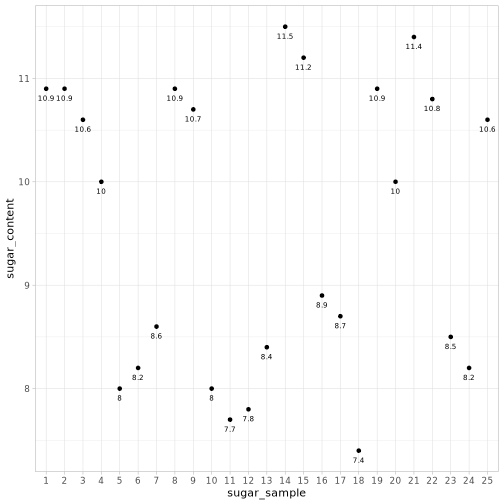
\includegraphics[width=1\linewidth]{note_usp657_files/figure-latex/unnamed-chunk-3-1}

\hypertarget{the-mmnl-class-of-models}{%
\paragraph{12.2 The MMNL Class of
Models}\label{the-mmnl-class-of-models}}

\(P_{qi}(\theta)=\int_{-\infty}^{+\infty}L_{qi}(\beta)f(\beta|\theta)d(\beta)\),
where \(L_{qi}(\beta)=\frac{e^{\beta'x_{qi}}}{\sum_je^{\beta'x_{qi}}}\)

\(P_{qi}\) is the probability that individual \(q\) chooses alternative
\(i\), \(x_{qi}\) is a vector of observed variables specific to
individual \(q\) and alternative \(i\), \(\beta\) represents parameters
which are random realizations from a density function \(f(.)\), and
\(\theta\) is a vector of underlying moment parameters characterizing
\(f(.)\).

Train (1986) and Ben-Akiva et al.~(1993) applied the mixed logit to
customer-level data, but considered only one or two random coefficients
in their specifications. Thus, they were able to use \emph{quadrature
techniques} for estimation.

The first applications to realize the full potential of mixed logit by
allowing several random coefficients simultaneously include Revelt and
Train (1998) and Bhat (1998b), both of which were originally completed
in the early 1996 and exploited the advances in simulation methods
(Train,2003;Bhat, 2005).

The MMNL model structure can be motivated from two very different (but
formally equivalent) perspectives (see Bhat, 2000a).

From an intrinsic motivation to allow flexible substitution patterns
across alternatives (\emph{error-components structure})

or from a need to accommodate unobserved heterogeneity across
individuals in their sensitivity to observed exogenous variables
(\emph{random coefficients structure}) or a combination of the two.

Assumption for \(f(.)\) are Normal, log-normal(\(\beta\) has to take the
same sign for every individual), triangular and uniform(bounded on both
sides;same sign for one or more coefficients), Rayleigh
distribution(same sign of coefficients for all decision makers).

the MMNL model represents a computationally efficient structure when the
number of error components (or factors) needed to generate the desired
error covariance structure across alternatives is much smaller than the
number of alternatives (see Bhat, 2003a,b

The MMNL model structure also serves as a comprehensive framework for
relaxing both the IID error structure as well as the response
homogeneity assumption.

\begin{longtable}[]{@{}lll@{}}
\toprule
\begin{minipage}[b]{0.13\columnwidth}\raggedright
\strut
\end{minipage} & \begin{minipage}[b]{0.39\columnwidth}\raggedright
MMNL model\strut
\end{minipage} & \begin{minipage}[b]{0.39\columnwidth}\raggedright
MNP model\strut
\end{minipage}\tabularnewline
\midrule
\endhead
\begin{minipage}[t]{0.13\columnwidth}\raggedright
capture random taste variations,substitution patterns\strut
\end{minipage} & \begin{minipage}[t]{0.39\columnwidth}\raggedright
flexible\strut
\end{minipage} & \begin{minipage}[t]{0.39\columnwidth}\raggedright
flexible\strut
\end{minipage}\tabularnewline
\begin{minipage}[t]{0.13\columnwidth}\raggedright
capture\strut
\end{minipage} & \begin{minipage}[t]{0.39\columnwidth}\raggedright
temporal correlation over time\strut
\end{minipage} & \begin{minipage}[t]{0.39\columnwidth}\raggedright
panel data\strut
\end{minipage}\tabularnewline
\begin{minipage}[t]{0.13\columnwidth}\raggedright
accommodate distributions\strut
\end{minipage} & \begin{minipage}[t]{0.39\columnwidth}\raggedright
non-normal\strut
\end{minipage} & \begin{minipage}[t]{0.39\columnwidth}\raggedright
only normal\strut
\end{minipage}\tabularnewline
\begin{minipage}[t]{0.13\columnwidth}\raggedright
understand the structure\strut
\end{minipage} & \begin{minipage}[t]{0.39\columnwidth}\raggedright
easier\strut
\end{minipage} & \begin{minipage}[t]{0.39\columnwidth}\raggedright
\strut
\end{minipage}\tabularnewline
\begin{minipage}[t]{0.13\columnwidth}\raggedright
estimate\strut
\end{minipage} & \begin{minipage}[t]{0.39\columnwidth}\raggedright
multidimensional integrals\strut
\end{minipage} & \begin{minipage}[t]{0.39\columnwidth}\raggedright
same\strut
\end{minipage}\tabularnewline
\begin{minipage}[t]{0.13\columnwidth}\raggedright
simulator\strut
\end{minipage} & \begin{minipage}[t]{0.39\columnwidth}\raggedright
arising from\strut
\end{minipage} & \begin{minipage}[t]{0.39\columnwidth}\raggedright
logit-smoothed Accept-Reject (AR)\strut
\end{minipage}\tabularnewline
\begin{minipage}[t]{0.13\columnwidth}\raggedright
code\strut
\end{minipage} & \begin{minipage}[t]{0.39\columnwidth}\raggedright
simple, straightforward\strut
\end{minipage} & \begin{minipage}[t]{0.39\columnwidth}\raggedright
\strut
\end{minipage}\tabularnewline
\begin{minipage}[t]{0.13\columnwidth}\raggedright
\strut
\end{minipage} & \begin{minipage}[t]{0.39\columnwidth}\raggedright
appealing and broad\strut
\end{minipage} & \begin{minipage}[t]{0.39\columnwidth}\raggedright
if number of normal random coefficients more than alternatives\strut
\end{minipage}\tabularnewline
\begin{minipage}[t]{0.13\columnwidth}\raggedright
dimensionality\strut
\end{minipage} & \begin{minipage}[t]{0.39\columnwidth}\raggedright
order of the number of random coefficients\strut
\end{minipage} & \begin{minipage}[t]{0.39\columnwidth}\raggedright
order of the number of alternatives\strut
\end{minipage}\tabularnewline
\bottomrule
\end{longtable}

\hypertarget{the-mixed-gev-class-of-models}{%
\paragraph{12.4 The Mixed GEV Class of
Models}\label{the-mixed-gev-class-of-models}}

There are instances when substantial computational efficiency gains may
be achieved using a MGEV structure.

It is possible that the utility of spatial units that are close to each
other will be correlated due to common unobserved spatial elements. A
common specification in the spatial analysis literature for capturing
such spatial correlation is to allow contiguous alternatives to be
correlated.

In the MMNL structure, such a correlation structure may require
multidimensional integration of the order of the number of spatial
units.

A carefully specified GEV model can accommodate the spatial correlation
structure within a closed-form formulation. However, the GEV model
structure of Bhat and Guo cannot accommodate unobserved random
heterogeneity across individuals.

The MGEV model involves multidimensional integration only of the order
of the number of random coefficients, while the MMNL model would entail
a multidimensional integration of the order of spatial units plus the
number of random coefficients.

A closed-form analytic structures should be used whenever feasible,
because they are always more accurate than the simulation evaluation of
analytically intractable structures. Superimposing a mixing structure to
accommodate random coefficients over a closed form analytic structure
that accommodates a particular desired inter-alternative error
correlation structure represents a powerful approach to capture random
taste variations and complex substitution patterns.

\hypertarget{dcm}{%
\subsection{DCM}\label{dcm}}

\texttt{Discrete\ choice\ methods\ with\ simulation}

\hypertarget{common-distributions}{%
\subsubsection{Common Distributions}\label{common-distributions}}

\begin{tabular}{ l|l|l|p{0.2\linewidth}|l }
   $D$   &$E;EX^2;V$&$f(x);F(x),P(X\le x)$&$MLE;T;I$&$M_x(t);M'(t);M''(t);M^n(t)$\\\hline
   
$Bern(p)$&$p$;$p$;$pq$&$p^xq^{1-x},x=1,0;0\le p\le1$&\shortstack{$\bar X$;$\sum x_i\sim Bin(n,p)$;$\frac1{pq}$;\\$Ep_{mle}=p$,$Vp_{mle}=\frac{pq}{n}$}&$pe^t+q$\\\hline

$Bino(n,p)$&$np$;$np(np+q)$;$npq$&$\binom{n}{x}p^x q^{n-x}$,$x=0,1..n;0\le p\le1$;&$\bar X$or$k\ge X_{(n)}$;$\sum x_i\sim Bino(n,p)$;$1/pq$&$(pe^t+q)^n$\\\hline

$Geom(p)$&$1/p$;${(p+2q)}/{p^2}$;$q/p^2$&$pq^{x-1}$,$x=1,2,..;0\le p\le1$;$1-q^x$&$1/\bar X$;$\sum x_i$;&$\frac{pe^t}{1-qe^t},t<-\ln{q}$;$\frac{pqe^t}{(1-qe^t)^2}$;$\frac{2pqe^t}{(1-qe^t)^3}-M'(t)$\\\hline

$NBino(r,p)$&$r/p$; ;$rq/p^2$;$0\le p\le1$&$\binom{x-1}{r-1}p^rq^{x-r}$,$x=r,r+1..$&$\bar X$;$\sum x_i$&$(\frac{pe^t}{1-qe^t})^r,t<\ln q$\\\hline

$HGeom(N,m,k)$&$\frac{km}N$;;$\mu\frac{(N-m)(N-k)}{N(N-1)}$;$N,m,k\ge0$ &${\binom{m}{x}\binom{N-m}{k-x}}/{\binom{N}{k}}$;&$m-(N-k)\le x\le m$\\\hline

$Pois(\mu)$&$\mu$;$\mu^2+\mu$;$\mu$;$\mu\ge0$&$\frac{\mu^x}{x!}e^{-\mu}$,$x=0,1..$;$e^{-\mu}\sum_{i=0}^x\frac{\mu^i}{i!}$&$\bar X$;$\sum x_i$;$\frac1\mu$;$P(x+1)=\frac\lambda{\lambda+1}P(x)$&$e^{\mu(e^t-1)}$;$\mu e^tM(t)$;$\mu e^t(1+\mu e^t)M(t)$\\\hline

$Unif(n)$&$\frac{n+1}2$;$\frac{(n+1)(2n+1)}{6}$;$\frac{n^2-1}{12}$&$\frac{1}n$,$x=1,2..n$,$n=b-a+1$;$\frac{x-a+1}n$&;$X_n$Comp&$\frac1n\sum_{i=1}^n{e^{ti}}$,$\frac{e^{at}-e^{(b+1)t}}{n(1-e^t)}$\\\hline

$Unif(a,b)$&$\frac{a+b}{2}$; ;$\frac{(b-a)^2}{12}$&$\frac{1}{b-a}$,$a\le x\le b$;$\frac{x-a}{b-a}$&$\min{x_{(1)},x_{(n)}}$;R ancillary&$\frac{e^{tb}-e^{ta}}{t(b-a)}$\\\hline

$Norm(\mu,\sigma^2)$&$\mu$;$\mu^2+\sigma^2$;$\sigma^2$&$\frac{1}{\sigma\sqrt{2\pi}} e^{-\frac{(x-\mu)^2}{2\sigma^2}}$,$\sigma>0$&\shortstack{$\bar X$,$\frac{\sum(x_i-\bar x)^2}n$;;$I_\mu=\frac1{\sigma^2}$,$I_{\sigma^2}=\frac1{2\sigma^4}$,$I_{\sigma}=\frac2{\sigma^2}$\\$E\hat\sigma^2_{mle}=\frac{(n-1)\sigma^2}{n}$,$V\hat\sigma_{mle}=\frac{2(n-1)\sigma^4}{n^2}$} &$e^{\mu t +\frac{\sigma^2t^2}2}$; $(\mu+\sigma^2t)M(t)$;$[(\mu+\sigma^2t)^2+\sigma^2]M(t)$\\\hline

$SNorm(0,1)$&$0$;$1$;$1$&$\frac{1}{\sqrt{2\pi}}e^{-\frac{x^2}2}$&&$e^{\frac{t^2}2}$\\\hline

$LNorm(\mu,\sigma^2)$&$e^{\mu+\frac{\sigma^2}2}$;$e^{2\mu+2\sigma^2}$;$E^2X(e^{\sigma^2}-1)$&$\frac{1}{x\sigma \sqrt{2\pi}}e^{\frac{-(\ln x-\mu)^2}{2\sigma^2}}$,$x\ge0$,$\sigma>0$&$\hat\mu=\frac1n\sum\ln x_i$,$\hat\sigma^2=\frac1n\sum\ln(x_i-\hat\mu)^2$&$EX^n=e^{n\mu+n^2\sigma^2/2}$\\\hline

$Cauchy(\theta,\sigma)$&&$\frac{1}{\pi\sigma}\frac1{1+(\frac{x-\theta}{\sigma})^2}$;;$\sigma>0$&=$t_1$;=$\frac{Z_1}{Z_2}$&\\\hline

$DExpo(\mu,\sigma^2)$&$\mu$;$\mu^2+2\sigma^2$;$2\sigma^2$&$\frac{1}{2\sigma} e^{-|\frac{x-\mu}{\sigma}|}$,$\sigma>0$;&$\hat\mu=median$,$\hat\sigma=\frac1n\sum|x_i|$&$\frac{e^{\mu t}}{1-\sigma^2t^2}$\\\hline

$Expo(\beta)$&$\beta$; ;$\beta^2$,$\beta>0$&$\frac1{\beta} e^{-\frac{x}\beta},x\ge0$;$1-e^{-\lambda x}$&\shortstack{$\frac1{\bar X}$;$\sum x_i$;$\frac1{\lambda^2}$;$E\lambda_{mle}=\frac{\lambda}{n-1}$,\\$V\lambda_{mle}=\frac{n^2\lambda^2}{(n-1)^2(n-2)}$,$V\lambda_{u}=\frac{\lambda^2}{n-2}$}&$\frac{\lambda}{\lambda-t},t<\lambda$,$\frac{1}{1-\beta t}$;$\frac{\beta}{(1-\beta t)^2}$;$\frac{2\beta^2}{(1-\beta t)^3}$\\\hline

$Gamm(\alpha,\beta)$&$\alpha\beta$; ;$\alpha\beta^2$;$\alpha,\beta>0$&$\frac{1}{\Gamma(a)\beta^{\alpha}}x^{a-1}e^{-x/\beta}$,$x\ge0$&$\prod x_i$,$\sum x_i$&$(\frac{1}{1-\beta t})^a, t <\frac1\beta$;$EX^n=\frac{\beta^n\Gamma(\alpha+n)}{\Gamma\alpha}$\\\hline

$Beta(a,b)$&$\frac{a}{a+b}$;$\frac{a(a+1)}{(a+b)(a+b+1)}$;$\frac{ab}{(a+b)^2(a+b+1)}$&$\frac{\Gamma(a+b)}{\Gamma(a)\Gamma(b)}x^{a-1}(1-x)^{b-1}$;$0\le x\le1$&$\alpha>0,\beta>0$&$B(\alpha,\beta)=\frac{\Gamma(\alpha)\Gamma(\beta)}{\Gamma(\alpha+\beta)}$,$x\in(0,1)$;$\frac{\Gamma(\alpha+n)\Gamma(\alpha+\beta)}{\Gamma(\alpha+\beta+n)\Gamma(\alpha)}$\\\hline

$\chi_p^2$&$p$;$2p+p^2$;$2p$&$\frac{1}{\Gamma \frac{p}2 2^{\frac{p}2}}x^{\frac{p}2-1}e^{-\frac{x}2}$,$x\ge0;p=1,2..$&;$\sum\ln x_i$;&$(1-2t)^{-p/2}, t<\frac12$\\\hline

$t_p$&$0,p>1$; ;$\frac{p}{p-2},p>2$&$\frac{\Gamma(\frac{p+1}2)}{\Gamma(\frac{p}2)\sqrt{p\pi}}(1+\frac{x^2}{p})^{-\frac{p+1}2}$&\\\hline

$F_{p,q}$&$\frac{q}{q-2},q>2$;;$2(\frac{q}{q-2})^2\frac{p+q-2}{p(q-4)},q>4$&$\frac{\Gamma(\frac{p+q}2)}{\Gamma(\frac{p}2)\Gamma (\frac{q}2)}(\frac{p}q)^{\frac{p}2}\frac{x^{\frac{p}2-1}}{(1+\frac{p}qx)^{\frac{p+q}2}}$,$x\ge0$&$F_{p,q}=\frac{\chi^2_p/p}{\chi^2_q/q}$;$F_{1,q}=t_q^2$&\\\hline

$Arcsine$&$\frac{1}2$; ;$\frac{1}8$&$\frac{1}{\pi\sqrt{x(1-x)}}$,$x\in[0,1]$;$\frac{1}{\pi\arcsin\sqrt x}$&&$Beta(\frac{1}2,\frac{1}2)$\\\hline

$Dirichlet$&$\frac{a_i}{\sum_ka_k}$$\sum_{i=1}^kx_i=1$;;$\frac{a_i(a_0-a_i)}{a_0^2(a_0+1)}$&$\frac1{B(a)}\Pi_{i=1}^kx_i^{a_i-1}$,$x\in(0,1)$&$B(a)=\frac{\Pi_{i=1}^k\Gamma(a_i)}{\Gamma(\sum_{i=1}^ka_i)}$&$Cov(X_i,X_j)=\frac{-a_ia_j}{a_0^2(a_0+1)}$,$a_0=\sum_{i=1}^ka_i$\\\hline

$Weibull(\gamma,\beta)$&\shortstack{$\beta^{1/\gamma}\Gamma(1+1/\gamma)$;;\\$\beta^{2/\gamma}[\Gamma(1+2/\gamma)-\Gamma^2(1+1/\gamma)]$}&\shortstack{$\frac\gamma\beta x^{\gamma-1}e^{-\frac{x^\gamma}\beta}$,$x\ge0$,$\gamma>0,\beta>0$;\\$1-e^{-(\frac{x}\beta)^\gamma}$}&$x^\gamma$,$\sum x^\gamma$,$\sum\ln x$&;;$\beta^{\frac{n}\gamma}\Gamma(1+\frac{n}\gamma)$\\\hline

$Pareto(\alpha,\beta)$&$\frac{\beta\alpha}{\beta-1}$,$\beta>1$;;$\frac{\beta\alpha^2}{(\beta-1)^2(\beta-2)}$,$\beta>2$&$\frac{\beta\alpha^\beta}{x^{\beta+1}}$;$1-(\frac{\alpha}{x})^\beta$,$x>\alpha$,$\alpha,\beta>0$&\shortstack{$\hat\alpha=\min x_i$,$\hat\beta=\frac{n}{\sum\ln(x_i/x_{(1)})}$;\\$\sum x_i$comp/suff;$1/\beta^2$}&
\end{tabular}

\end{document}
